\documentclass{ctexart}
\usepackage{geometry}
\usepackage{diagbox}
\usepackage{graphicx}
\usepackage{subfigure}
\usepackage{amsmath}
\usepackage{amssymb}
\usepackage{indentfirst}
\usepackage{xfrac}
\usepackage{color}
\usepackage[table]{xcolor}
\usepackage{multirow}
\usepackage{titlesec}
\usepackage{bm}
\usepackage{caption}
\title{UP主粉丝数的影响因素分析}
\author{CDA小组}
\date{}
\begin{document}
\maketitle
\begin{abstract}
    这里是摘要
\end{abstract}
\section{背景介绍}
Bilibili视频网站(下文简称B站)在近年愈发受到年轻人的欢迎,数量庞大的UP主群体为B站的视频生态的多样性做出了
非常大的贡献。在庞大的UP主群体之下,UP主的粉丝数也有显著的差异。本研究旨在通过研究各种影响因素与UP主的粉丝
数量的分层不同带来的影响。\\
\indent 本次研究的数据来源于ifans网站,网站上提供了粉丝量、最近更新时间、分区、视频数、
充电数、近8篇平均视频投币数、近8篇平均视频弹幕数、近8篇平均视频收藏数、近8篇平均视频点赞数、
近8篇平均视频播放数、近8篇平均视频评论数、近8篇平均视频分享数数据、性别数据,本研究将所有变量均放入模型中进行研究,
同时研究是否能够有减少变量的方法。本研究凭借网站上的粉丝数量分区,
将粉丝量的分区分为“<10万”,“10万~50万”,“50万~100万”,“>100万”四个分区,作为后续分类型数据分析的基础。\\
\indent 由于不同分区的UP主人数差异较大,本研究采用回溯性研究方法,即在四个粉丝量的分区分别抽取250个UP主的数据
进行研究分析。
\section{数据预处理}
由于每个变量的单位相差较大,为了避免单位造成的影响,本研究将所有非分类型数据进行归一化处理。
由于选择的解释变量均为非负数据,为保持这一性质,采用以下的归一化方法。
\begin{equation}
    \tilde{x} = \frac{x-\alpha}{\beta - \alpha}
\end{equation}
其中$\alpha$,$\beta$分别为本解释变量中的最大值与最小值。
\section{探索性数据分析}
\subsection{数据可视化}
首先,作出各类数据之间相关系数的热量图:
\begin{figure}[htbp]
    \centering
    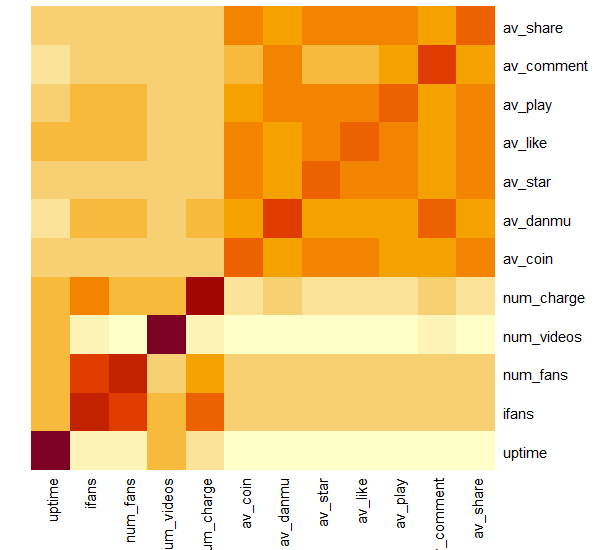
\includegraphics[width=0.40\textwidth]{EDA/Heatmap.png}
    \caption{Heatmap for Correlation}
\end{figure}\\
\indent 由热量图可见,右上角各种平均的线性相关性较强。由于作出Scatter Plot Matrix时,如果变量过多,则容易显示不清楚,因此
选择近8篇平均投币数和近8篇平均点赞数作为各种平均的代表绘制Scatter Plot Matrix。
\begin{figure}[htbp]
    \centering
    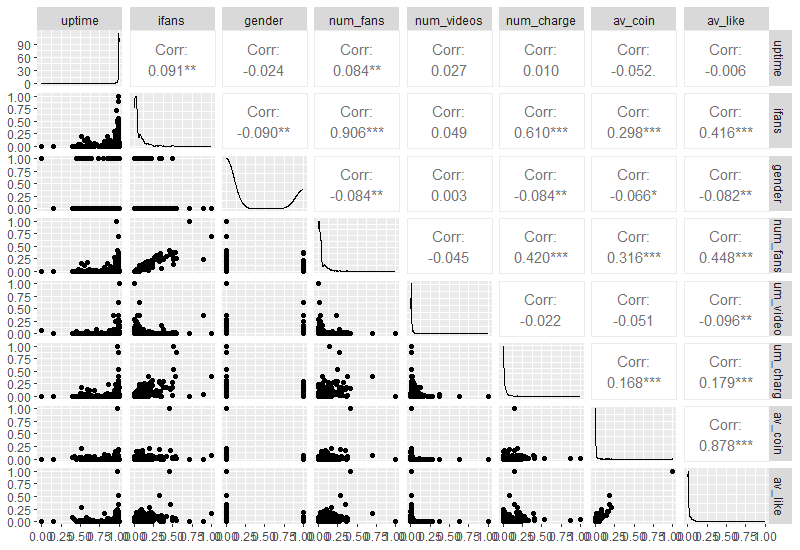
\includegraphics[width=0.60\textwidth]{EDA/Spm.png}
    \caption{Scatter Plot Matrix}
\end{figure}\\
\indent 由Scatter Plot Matrix可见,各类数据间普遍具有一定的相关性,这说明对这些数据建立模型进行分析应该会有一定的效果。同时,由每个变量的核密度
估计可见,各个解释变量是明显右偏的,这说明B站的UP主存在一定的少部分UP主占据了极大的资源的效应。\\
\indent 通过Scatter Plot Matrix,作出两大分区变量粉丝量与性别和与这两个因素有显著作用的的变量之间的箱型图,观察这些因素对
两大分类型变量的影响。
\begin{figure}[htbp]
    \begin{minipage}[t]{0.48\textwidth}
        \centering
        \includegraphics[width=\textwidth]{EDA/av_like_gender_boxplot.png}
        \caption{各性别平均点赞数}
    \end{minipage}
    \begin{minipage}[t]{0.48\textwidth}
        \centering
        \includegraphics[width=\textwidth]{EDA/num_charges_gender_boxplot.png}
        \caption{各性别充电数}
    \end{minipage}
\end{figure}
\begin{figure}[htbp]
    \begin{minipage}[t]{0.48\textwidth}
        \centering
        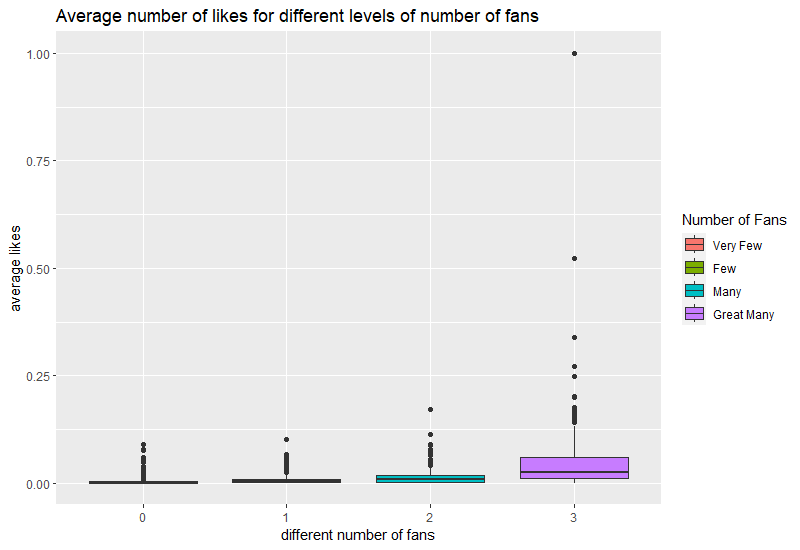
\includegraphics[width=\textwidth]{EDA/av_like_fans_boxplot.png}
        \caption{各粉丝量平均点赞数}
    \end{minipage}
    \begin{minipage}[t]{0.48\textwidth}
        \centering
        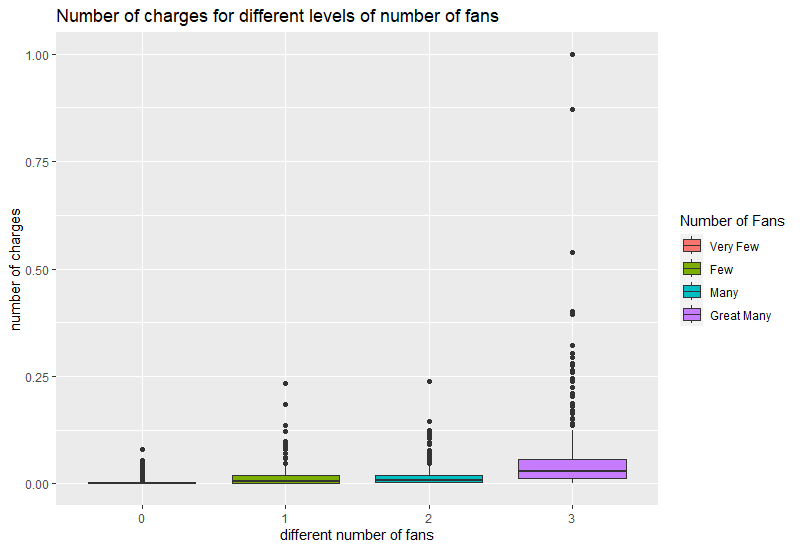
\includegraphics[width=\textwidth]{EDA/num_charge_fan_boxplot.png}
        \caption{各粉丝量充电数}
    \end{minipage}
\end{figure}\\
\indent 由图可见,对于部分解释变量,其对不同性别确实有显著的影响;对于平均点赞数和充电数而言,均表现为男性的
离群值点远大于女性的特点。而诸多解释变量对于粉丝量也有显著的作用,与上述分析相似的,对于粉丝量较少的三类,实际上
两个变量的表现较为相似,而粉丝量大于100万的样本,在点赞量和充电数上,无论是平均值还是数量高的值都明显多于前三类。
这映照了之前认为的少部分UP主获得了最多的关注的同时,也按时是否需要优化分区结构,能够获得更好的效果。\\
\\
\indent 由于解释变量仍较多,并且从Scatter Plot Matrix可以看出部分解释变量之间存在较为显著的线性相关性,
因此考虑是否能对解释变量进行一定程度的筛选。下面考虑利用主成分分析(PCA)和LASSO两种方法对是否能够减少解释变量数量进行分析。
\subsection{主成分分析}
对归一化后的连续型解释变量进行主成分分析,所得肘图如下图:
\begin{figure}[htbp]
    \centering
    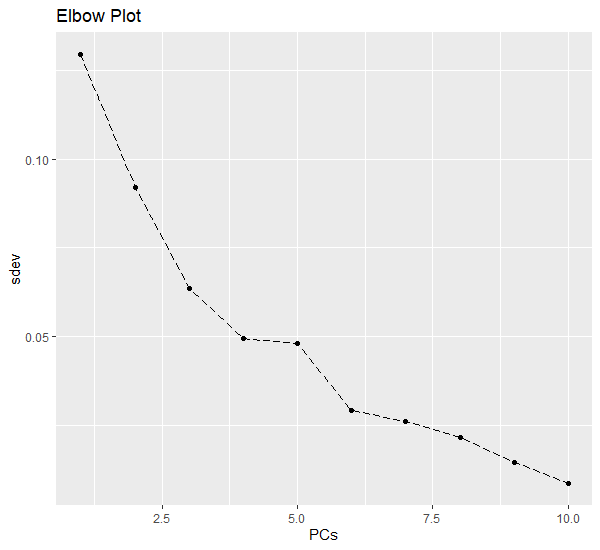
\includegraphics[width=0.45\textwidth]{EDA/PCA_elbow.png}
    \caption{PCA肘图}
\end{figure}\\
\indent 由肘图可见,实际上PCA的效果并不好,在拐点后方程下降速度仍较为显著,
并且拐点处的方差仍较大。如果要保留99\%的信息量,则可舍弃最后两个主成分;如果要保留95\%的信息量,则可舍弃最后四个主成分。一定程度上起到了降维
的效果。PCA的旋转矩阵如下表:
\begin{table}[htbp]
    \centering
    \begin{tabular}{|c|c|c|c|c|c|c|c|c|c|c|}
    \hline
            & PC1   & PC2   & PC3   & PC4   & PC5   & PC6   & PC7   & PC8   & PC9   & PC10  \\ \hline
    uptime  & -0.17 & 0.97  & 0     & 0.11  & -0.08 & 0.04  & -0.03 & 0.01  & -0.02 & -0.01 \\ \hline
    videos  & -0.04 & 0     & -0.03 & 0.55  & 0.83  & -0.04 & -0.04 & 0     & -0.01 & 0.01  \\ \hline
    charge  & 0.15  & 0.07  & -0.93 & -0.29 & 0.17  & 0.04  & -0.01 & 0     & -0.01 & 0     \\ \hline
    coin    & 0.23  & 0.07  & 0.08  & -0.07 & 0.1   & 0.21  & 0.46  & -0.36 & 0.33  & -0.65 \\ \hline
    danmu   & 0.51  & 0.01  & -0.17 & 0.57  & -0.35 & -0.19 & 0.37  & 0.3   & -0.01 & 0.08  \\ \hline
    star    & 0.3   & 0.08  & 0.16  & -0.2  & 0.16  & 0.09  & 0.31  & -0.26 & -0.78 & 0.17  \\ \hline
    like    & 0.32  & 0.12  & 0.14  & -0.19 & 0.14  & -0.13 & 0.09  & -0.32 & 0.51  & 0.65  \\ \hline
    play    & 0.48  & 0.12  & 0.14  & -0.19 & 0.11  & -0.58 & -0.47 & 0.06  & -0.05 & -0.35 \\ \hline
    comment & 0.31  & -0.03 & -0.07 & 0.33  & -0.21 & 0.49  & -0.56 & -0.44 & -0.05 & 0.01  \\ \hline
    share   & 0.34  & 0.08  & 0.2   & -0.23 & 0.2   & 0.56  & -0.07 & 0.65  & 0.1   & 0.03  \\ \hline
    \end{tabular}
    \caption{PCA旋转矩阵}
\end{table}\\
\indent 由旋转矩阵可见,实际上PCA的解释性较差。又由于本研究主要为解释性研究,因此如果采用PCA后的主成分进行分析,
最后会导致解释性较差,所以将舍弃PCA部分的结果。
\subsection{LASSO}
利用LASSO将所有解释变量放入模型中,分别对粉丝量(分类型)作多分类变量逻辑回归与对粉丝量(连续型)作广义线性回归,得到
均方误差随正则项的变化分别如下两图。
\begin{figure}[htbp]
    \begin{minipage}[t]{0.48\textwidth}
        \centering
        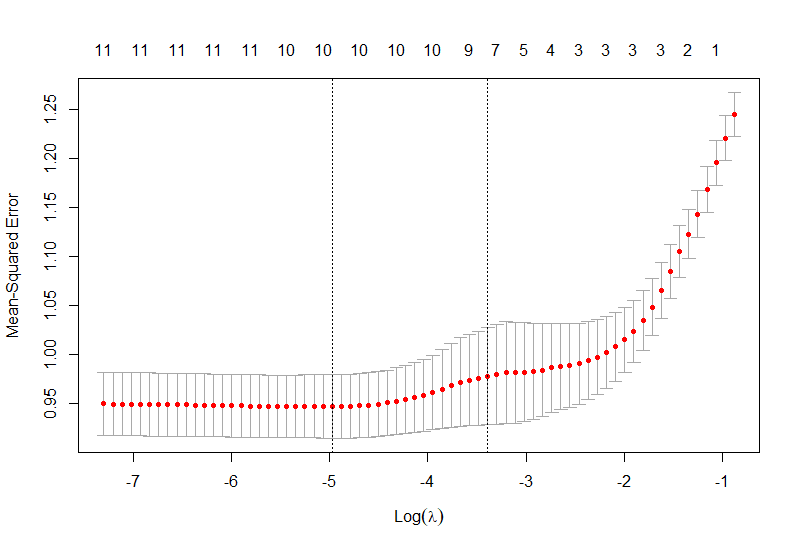
\includegraphics[width=\textwidth]{EDA/lasso_multinomial.png}
        \caption{多分类逻辑回归}
    \end{minipage}
    \begin{minipage}[t]{0.48\textwidth}
        \centering
        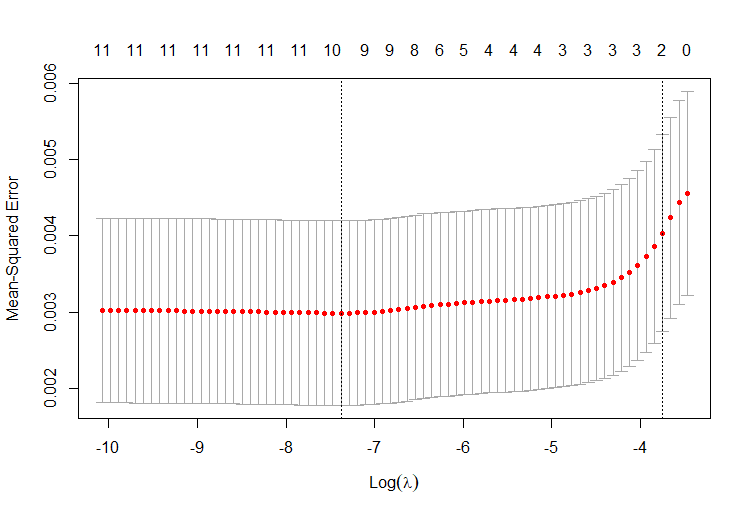
\includegraphics[width=\textwidth]{EDA/lasso_continuous.png}
        \caption{连续型线性回归}
    \end{minipage}
\end{figure}\\
\indent 所得在让均方误差最小的正则项系数与在1个标准差意义下的正则项系数如下表,其中进行多分类逻辑回归得到4个返回的$\lambda$值,
筛选出效果较好的值对应的系数:
\begin{table}[htbp]
    \centering
    \begin{tabular}{ccccc}
    \hline
    \multirow{2}{*}{Name} & \multicolumn{2}{c}{Multinomial} & \multicolumn{2}{c}{Continuous} \\ \cline{2-5} 
                          & min            & 1se            & min            & 1se           \\ \hline
    Intercept             & 8.76           & 5.26           & -0.03          & 0.04          \\
    uptime                & -8.16          & -5.69          & 0.05           & 0             \\
    gender                & 0.08           & 0.15           & 0              & 0             \\
    videos                & -1.08          & 0              & 0              & 0             \\
    charge                & -54.93         & -20.74         & 0.34           & 0.05          \\
    coin                  & 0              & 0              & -0.3           & 0             \\
    danmu                 & 0              & 0              & 0.09           & 0             \\
    star                  & 8.08           & 0              & -0.11          & 0             \\
    like                  & -73.91         & -21.17         & 0.66           & 0             \\
    play                  & -13.79         & 0              & 0.2            & 0.1           \\
    comment               & -1.07          & 0              & -0.06          & 0             \\
    share                 & 22.47          & 0              & -0.16          & 0             \\ \hline
    \end{tabular}
    \caption{正则后系数表}
\end{table}\\
\indent 由上表可见,使用LASSO多类别逻辑回归和线性回归得到的系数有较为明显的区别,因此说明经过将粉丝量分类,得到了
不同的回归结果,有不同的解释效应。因此,在进行多分类逻辑回归会得到直接线性回归不同的结果。由于两个1个标准差内的结果
都省略了过多的变量,可能造成解释能力不足,因此在进行多分类逻辑回归时,考虑舍弃投币数和弹幕数两个变量。
\end{document}